\newpage
\appendix
\newcommand{\mytoptitlebar}{
  %\hrule height 4
  \noindent\rule{\textwidth}{4pt}
  \vskip 0.16in
  %\vspace{0.1in}
  %\vskip -\parskip%
}
\newcommand{\mybottomtitlebar}{
  %\vskip 0.01in
  %\vskip -\parskip
  %\hrule height 1
  \noindent\rule{\textwidth}{1.pt}
  %\vskip 0.05in%
}


\mytoptitlebar
\begin{center}
	{\Large\bf Supplemental Material: Computational Budget Should Be Considered in Data Selection }
\end{center}
\mybottomtitlebar
\vskip 0.2in

% \section*{Appendix}
In this appendix, we provide comprehensive additional materials to supplement the main text. The contents include:
\begin{itemize}
\item \textbf{Broader impacts (Section~\ref{appendix:impacts}):} A discussion on the broader implications of our research.
\item \textbf{Experimental setting and implementation details (Section~\ref{appendix:experimental_settings}):} Detailed information on the experimental settings and implementation details.
\item \textbf{Log-linear surrogate of compute-constrained training loss (Section~\ref{appendix:surrogate}):} Explanation of approximating \(\mathcal{L}_{\mathrm{trn}}(\mathbf{u},\mathbf{m})\) by the scale-dependent surrogate \(l(|\mathbf{m}|)\), its log-space interpolation, and fitting procedure.
\item \textbf{Visualizations on truncated Gaussian distribution (Section~\ref{appendix:gaussian}):} Detailed visualization on the truncated Gaussian distribution.
\item \textbf{Additional experimental results (Section~\ref{appendix:additional-results}):} MNIST experiments varying the total compute budget to compare random, PBCS, CADS-E, and Bilevel-CADS. The results show that our method consistently achieves the highest accuracy (Table~\ref{tab:mnist_vary_budget}). 
\item \textbf{Time efficiency analysis (Section~\ref{appendix:time_efficiency}):} Benchmarking of average training and sampling runtimes on representative hardware.
\item \textbf{Scalability to other bilevel optimization problems (Section~\ref{appendix:scala2other}):} Discussion on the applicability conditions, loss estimation accuracy, and a validation framework for applying CADS to new domains.
\item \textbf{Limitations and future work (Section~\ref{appendix:limitation}):} Analysis of the limitations in our current framework, and plans for future improvements.
\item \textbf{Licenses for existing assets (Section~\ref{appendix:license}):} Acknowledgment and respect for the licenses and terms of use of datasets and code libraries utilized in our research.
\end{itemize}

\section{Broader impacts}
\label{appendix:impacts}
This work introduces CADS, a compute-aware data selection algorithm that dynamically adapts the training data budget according to available computational resources. By optimizing data efficiency relative to compute constraints, CADS significantly reduces the computational overhead of training deep learning models without sacrificing performance. This advancement enables more accessible and environmentally sustainable machine learning research and deployment, particularly in scenarios constrained by limited hardware resources.
The method’s potential to lower energy consumption during model training aligns with broader community efforts towards greener AI, contributing to reductions in carbon footprint and operational costs. Additionally, CADS facilitates democratization of deep learning by empowering researchers and practitioners with modest resources to train competitive models.
However, as with any automation that accelerates model training, there exist potential risks, including the possibility of speeding up the development of models with harmful biases, privacy vulnerabilities, or malicious intent if not applied responsibly. We stress the importance of ethical use and compliance with community norms and regulatory standards when deploying such techniques.
Overall, CADS represents a step forward in efficient and responsible machine learning practices, promoting sustainability and equitable access within the deep learning community.
\section{Experimental setting and implementation details}
\label{appendix:experimental_settings}
In this section, we detail the protocols and implementation specifics underlying all our evaluations. 
All experiments were run on a single machine equipped with an NVIDIA A100 80 GB GPU under CUDA 12.6 and NVIDIA driver 470.199.02, using PyTorch 2.5.1.

\subsection{Exploratory experiment on spectrum bias}
\label{appendix:exp-spectrum-bias}

To isolate the effect of spectral content on generalization, we generate two synthetic datasets with identical noise level \(\sigma=0.1\) but different frequency composition.

\paragraph{Data generation.} We sample \(N=50{,}000\) inputs for each group; for the low-frequency dataset (Group A) we set \(y = x + \mathcal{N}(0,\sigma^2)\), and for the high-frequency dataset (Group B) we set \(y = x + \frac{\sin(\pi x)}{\pi x} + \mathcal{N}(0,\sigma^2)\). A fixed validation set of 10,000 points is used to track generalization error.

\paragraph{Model and training.}  
Each model is a three-layer MLP (100–100 hidden units, ReLU). We train for 160 steps using Adam (learning rate \(3\times10^{-4}\)) and batch size 1000. After every parameter update, we compute the MSE on the validation set and log the result. The different positions on the x-axis in Figure~\ref{fig:impact} correspond to these intermediate results recorded during the training process.

\subsection{Small-scale validation}  
\label{appendix:small-scale-validation}   
We validate CADS on a reduced‐scale MNIST classification task using a simple convolutional network. All experiments use a fixed training set of 1,000 examples and batch size 1,000. We optimize under an epoch‐based budget of 20 epochs. The selection parameters $\bm{s}\in\mathbb{R}^{|D|}$ are initialized as  
\(
\bm{s} \;=\; v \cdot \bm{1}, 
\quad v \in \{0.2,\,0.4,\,0.6,\,0.8\},
\quad \bm{1}\in\mathbb{R}^{|D|} \text{ is the all-ones vector}.
\)
We solve the bilevel problem with Adam for both the network parameters $\theta$ (learning rate $5\times10^{-3}$) and the selection weights $\bm{s}$ (learning rate $5\times10^{-2}$). The outer loop runs for 300 iterations with variance reduction and gradient clipping enabled.

\paragraph{Network architecture.}  
We employ a simple convolutional model: two convolutional layers with $5\times5$ kernels and channel counts $\{32,64\}$, each followed by ReLU and optional $2\times2$ max‐pooling; the feature map is flattened ($4\times4\times64=1024$ units) and passed through a fully connected layer of 128 units with ReLU; a final linear layer outputs class logits. Input normalization by fixed mean and standard deviation is applied when enabled. No dropout is used.  

\subsection{Heterogeneous data sources: small‐scale experiments on CIFAR‐10}  
\label{appendix:heterogeneous-cifar10}  
We evaluate CADS‐S on a grouped CIFAR‐10 variant with five demographic groups and up to $90\%$ label noise. All experiments use the full training set (no limit) with batch size $256$. We allocate an epoch‐based compute budget of $2$ to $5$ epochs. The selection parameter $\bm{s}$ is initialized to $0.5\cdot \bm{1}^{|D|}$. We solve the bilevel problem with Adam for both network parameters $\theta$ (learning rate $5\times10^{-3}$) and selection weights $s$ (learning rate $5\times10^{-2}$), over $100$ outer iterations with variance reduction and gradient clipping. We adopt the standard ResNet-$18$ backbone for all runs.
\subsection{Heterogeneous data sources: scaling to larger datasets}
\label{appendix:heterogeneous-domainnet}

We evaluate CADS‐S on DomainNet with \(6\) groups using the full training set and batch size \(1024\). We allocate an epoch‐based compute budget of \(10\) epochs. The selection parameters $\bm{s}\in\mathbb{R}^{|D|}$ are initialized as  
\(
\bm{s} \;=\; v \cdot \bm{1}, 
\quad v \in \{0.2,\,0.4,\,0.6,\,0.8\},
\quad \bm{1}\in\mathbb{R}^{|D|} \text{ is the all-ones vector}.
\) We solve the bilevel problem with Adam for both network parameters \(\theta\) (learning rate \(5\times10^{-3}\)) and selection weights $\bm{s}$ (learning rate \(5\times10^{-2}\)), over \(100\) outer iterations with variance reduction and gradient clipping. We adopt the standard ResNet-\(18\) backbone for all runs.

\paragraph{DomainNet dataset.}  
DomainNet comprises over \(0.5\) million images across six visual domains: Real, Sketch, Clipart, Painting, Infograph, and Quickdraw (As shown in Fig.~\ref{fig:domainnet}). In our setup, we treat the Real domain as a high‐quality source but include only \(10{,}000\) samples from it to simulate limited access; the other five domains are used in full. 

\begin{figure}[!htbp]
\centering
\begin{minipage}[b]{0.27\textwidth}
  \centering
  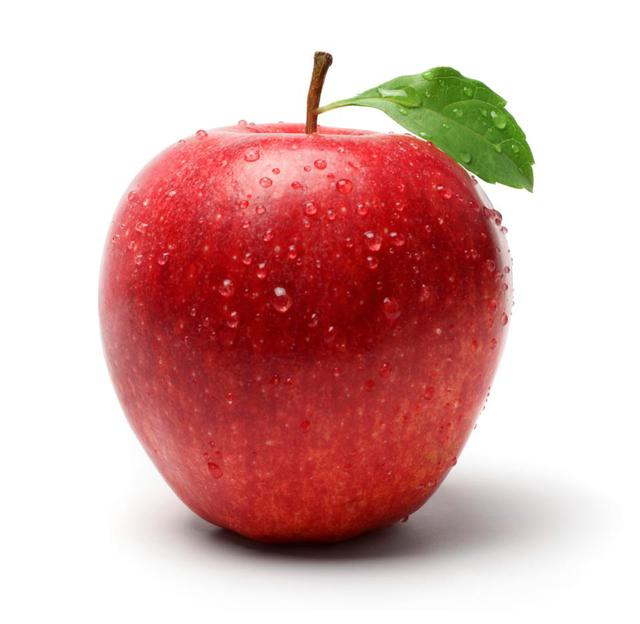
\includegraphics[width=\linewidth]{pics/domainnet/real_009_000025.jpg}
  \\(a) Real
\end{minipage}\hfill
\begin{minipage}[b]{0.27\textwidth}
  \centering
  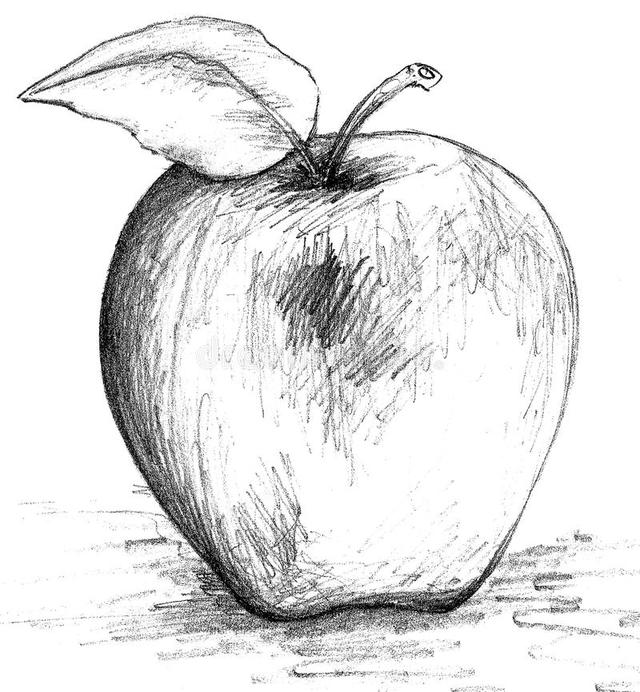
\includegraphics[width=0.8\linewidth]{pics/domainnet/sketch_009_000012.jpg}
  \\(b) Sketch
\end{minipage}\hfill
\begin{minipage}[b]{0.27\textwidth}
  \centering
  
\includegraphics[width=\linewidth]{pics/domainnet/clipart_009_000013.jpg}
  \\(c) Clipart
\end{minipage}

\vskip 1em

\begin{minipage}[b]{0.27\textwidth}
  \centering
  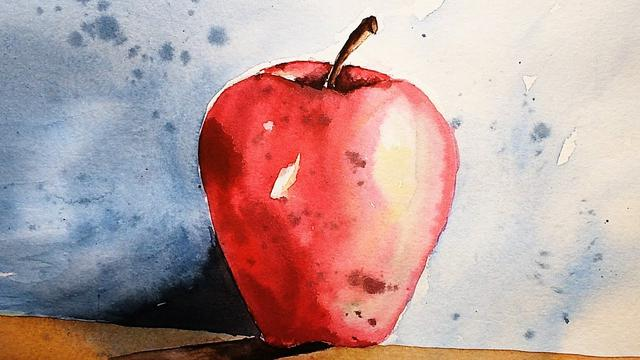
\includegraphics[width=\linewidth]{pics/domainnet/painting_009_000004.jpg}
  \\(d) Painting
\end{minipage}\hfill
\begin{minipage}[b]{0.27\textwidth}
  \centering
  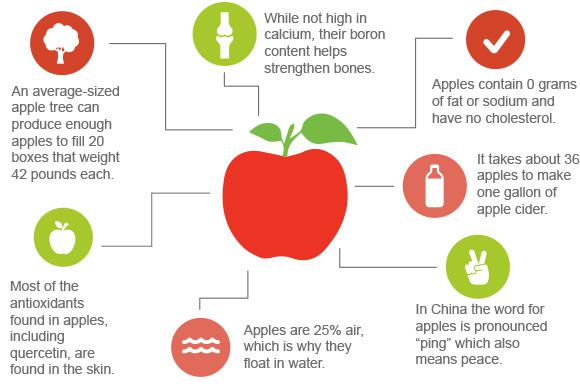
\includegraphics[width=\linewidth]{pics/domainnet/infograph_009_000020.jpg}
  \\(e) Infograph
\end{minipage}\hfill
\begin{minipage}[b]{0.3\textwidth}
  \centering
  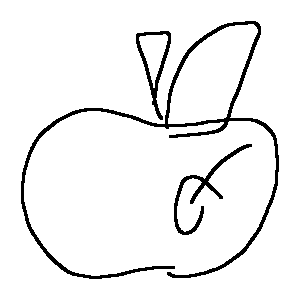
\includegraphics[width=0.7\linewidth]{pics/domainnet/quickdraw.png}
  \\(f) Quickdraw
\end{minipage}

\caption{Representative examples from the DomainNet domains: Real, Sketch, Clipart (top row); Painting, Infograph, Quickdraw (bottom row).}
\label{fig:domainnet}
\end{figure}

\subsection{Instruction tuning tasks: small-scale experiments}
\label{appendix:instruction-tuning-small}

We evaluated our CADS‐S approach on instruction fine‐tuning tasks using the GPT-2 model~\cite{Radford2019LanguageMA}. The dataset consists of two heterogeneous data sources: (i) \textbf{Alpaca-GPT4}~\cite{alpaca-gpt4}, a high-quality dataset from GPT-4-generated instructions, from which we sample \(1{,}000\) examples to simulate the rarity of premium data sources in practical scenarios; (ii) \textbf{Alpaca}~\cite{alpaca}, a larger dataset containing \(9{,}000\) examples, representing standard-quality data. The total compute budget varies within the range \([1\times10^{4},5\times10^{4}]\) sample usages. 
The selection weight \(s\) is initialized to \(0.5\cdot \bm{1}^{|D|}\). We solve the bilevel problem with AdamW for both model parameters \(\theta\) (learning rate \(1\times10^{-5}\)) and selection weights $\bm{s}$ (learning rate \(5\times10^{-2}\)). We adopt the GPT-2 backbone with maximum sequence length \(1024\) for all runs.

\paragraph{Data preprocessing.}  
Raw instruction–response samples are loaded from JSON or JSONL files and consolidated into a flat record list. A pretrained tokenizer is initialized and extended to include five special markers: a padding token, an end‐of‐sequence token, and three role‐demarcation tokens (<|system|>, <|user|>, <|assistant|>). Each record is then serialized into a single text sequence by:
\begin{enumerate}
  \item Emitting the system token, followed by the system‐level directive, and two line breaks.
  \item Emitting the user token, followed by the instruction text (and any optional input), and two line breaks.
  \item Emitting the assistant token, followed by the target response, and terminating with the end‐of‐sequence token.
\end{enumerate}
The concatenated text is first tokenized without truncation to measure its length; any example that exceeds the maximum allowed token count is discarded. The remaining examples are split into training, validation, and test subsets according to either explicitly provided sizes or a default 90/5/5 ratio.
At training time, each sequence is tokenized with truncation to the maximum length, producing token identifiers and attention masks. All token positions corresponding to the system and user segments are assigned an ignore index in the label sequence so that only assistant‐response tokens contribute to the loss. A bespoke collation routine then pads every batch to the length of its longest sequence, using the padding token for inputs, zeros for masks, and the ignore index for both prompt and padding positions in the labels. 

\subsection{Instruction tuning tasks: scaling to additional datasets}

We extended our evaluation to 13 distinct instruction‐following corpora, drawing ten thousand examples from each. These included the original AlpacaGPT4 benchmark\cite{alpaca-gpt4}, the SlimOrca set\cite{slimorca}, the Alpaca collection\cite{alpaca}, the GPTeacher suite\cite{gpteacher}, and nine multilingual variants of the Alpaca data. In total, approximately 130 000 samples were processed with the identical tokenization, formatting, filtering, and batch‐collation pipeline described above. The complete list of datasets, along with their sizes and licenses, is summarized in Table~\ref{tab:stat_data}.

\begin{table}[h]
    \centering
    \renewcommand\arraystretch{1.3}
    \setlength{\tabcolsep}{1.5mm}
    \begin{tabular}{lcr}
        \toprule
        Dataset & Size & License \\
        \midrule
        AlpacaGPT4~\citep{alpaca-gpt4}        & 52K & Apache-2.0 \\
        SlimOrca~\citep{slimorca}            & 518K & MIT        \\
        GPTeacher~\citep{gpteacher}          & 89K & MIT        \\
        Alpaca~\citep{alpaca}                & 52K & Apache-2.0 \\
        \midrule
        Alpaca-es\tablefootnote{\url{https://huggingface.co/datasets/bertin-project/alpaca-spanish}} & 52K & CC-BY-4.0        \\
        Alpaca-de\tablefootnote{\url{https://huggingface.co/datasets/mayflowergmbh/alpaca-gpt4_de}}     & 50K & Apache-2.0       \\
        Alpaca-ja\tablefootnote{\url{https://huggingface.co/datasets/fujiki/japanese_alpaca_data}}    & 52K & CC-BY-NC-SA-4.0  \\
        Alpaca-ko\tablefootnote{\url{https://huggingface.co/datasets/Bingsu/ko_alpaca_data}}         & 50K & CC-BY-NC-4.0     \\
        Alpaca-ru\tablefootnote{\url{https://huggingface.co/datasets/IlyaGusev/ru_turbo_alpaca}}      & 30K & CC-BY-4.0        \\
        Alpaca-it\tablefootnote{\url{https://huggingface.co/datasets/mchl-labs/stambecco_data_it}}    & 52K & CC-BY-NC-SA-4.0  \\
        Alpaca-fr\tablefootnote{\url{https://huggingface.co/datasets/jpacifico/French-Alpaca-dataset-Instruct-55K}} & 55K & Apache-2.0       \\
        Alpaca-zh\tablefootnote{\url{https://huggingface.co/datasets/llm-wizard/alpaca-gpt4-data-zh}}  & 49K & CC-BY-4.0        \\
        Alpaca-pt\tablefootnote{\url{https://huggingface.co/datasets/dominguesm/alpaca-data-pt-br}}   & 52K & CC-BY-NC-4.0     \\
        \bottomrule
    \end{tabular}
    \vskip 0.2in
    \caption{Summary of high‐quality instruction‐tuning datasets (top) and multilingual Alpaca variants (bottom).}
    \label{tab:stat_data}
\end{table} 

\section{Log-linear surrogate of compute-constrained training loss}
\label{appendix:surrogate}
\subsection{Data Collection}
We collect estimates of the $K$-step (“compute-constrained”) training loss
\(
  \mathcal{L}_{\mathrm{trn}}(\theta;|m|)
\)
at a range of subset sizes $|m|$.  By default we choose nine relative fractions
$\{0.01,0.02,0.05,0.1,0.3,0.5,0.7,0.9\}$ of the full training set
(clamped to at least 50 examples on MNIST or the configured batch‐size otherwise).
For each size we train for a total compute budget $N$ (so that each inner training run sees roughly the same total number of gradient steps), and record the final training loss. We then summarize each size by its empirical~$\ell_j$.

\subsection{Surrogate model choice}
We set \(\varepsilon=10^{-10}\) and fit the transformed log‐loss
\(\log\bigl(l(|m|)+\varepsilon\bigr)\) using two options:
\begin{itemize}
  \item \textbf{Linear:}  
    \(\log\bigl(l(|m|)+\varepsilon\bigr)=k\,|m|+b\).
  \item \textbf{Cubic spline interpolation:}  
    fit a cubic spline through the points 
    \(\bigl(|m_{j}|,\log(l(|m_{j}|)+\varepsilon)\bigr)\), 
    yielding a piecewise‐cubic function \(\hat f(|m|)\).
\end{itemize}
After fitting in log‐space, we recover the original‐scale surrogate via
\(\displaystyle l(|m|)=\exp\bigl(\hat f(|m|)\bigr)\).
Figure~\ref{fig:appendix-fits} overlays these fitted curves on the empirical training‐loss measurements. The cubic spline interpolation achieves a noticeably lower MSE, motivating its use when maximum fidelity is desired, while the linear surrogate offers simplicity and a closed‐form gradient. 
\textbf{Since CADS never computes \(\partial l(|m|)/\partial |m|\), we exclusively employ the cubic spline interpolation due to its superior fit.}

\begin{figure}[t]
  \centering
  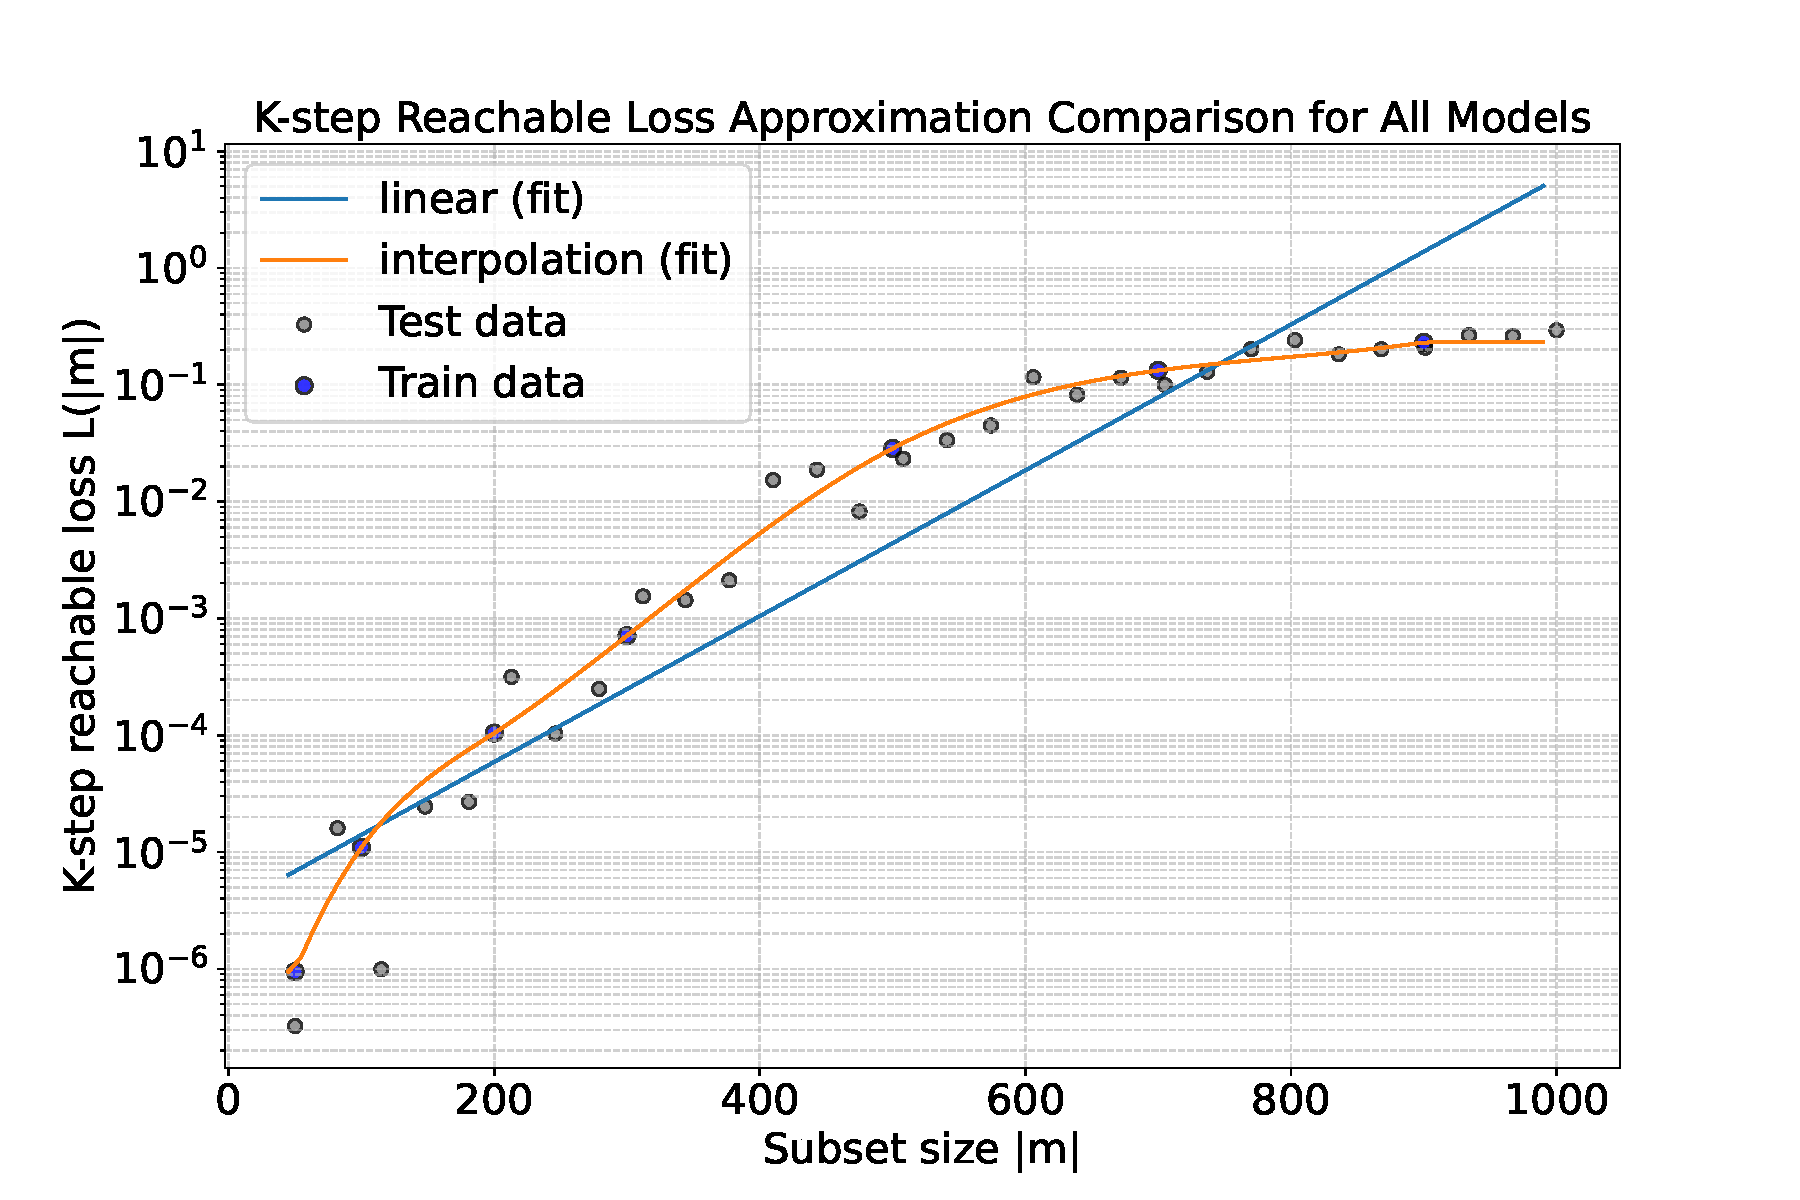
\includegraphics[width=0.8\linewidth]{pics/all_models_comparison.pdf}
  \caption{All‐models comparison of the K‐step reachable loss as a function of subset size $|m|$. Blue circles denote observed mean loss on training subsets; gray squares denote observations on held‐out test subsets. Solid curves show the fitted approximation functions for each candidate model. The vertical axis is plotted on a logarithmic scale.}
  \label{fig:appendix-fits}
\end{figure}


\subsection{Analysis of Sampling Efficiency for Loss Estimation}
\label{appendix:sampling_efficiency}

To evaluate the sample efficiency of our loss estimation method, we conducted an analysis to determine the minimum number of subset samples (\(K\)) required for reliable interpolation.

\paragraph{Experimental Design}
On the CIFAR-10 dataset with a ResNet-18 model, we evaluated the loss estimator's performance under varying sampling densities, where \(K \in \{4, 5, 6, 7, 8\}\). For each value of \(K\), we sampled \(K\) distinct subset sizes to train corresponding models, yielding \(K\) pairs of (size, loss) data points. These points were used to fit the loss estimator. Subsequently, we tested each fitted estimator on a held-out set of 100 separately sampled (size, loss) pairs to measure its interpolation accuracy.

\paragraph{Results}
The results, summarized in Table~\ref{tab:sampling_efficiency_mse}, demonstrate that the estimator's performance improves significantly up to \(K=5\) sampling points, after which the returns diminish. This indicates that our method is highly sample-efficient. Notably, increasing \(K\) further (e.g., \(K=7\)) can slightly degrade performance, likely due to overfitting the estimator to a specific set of sample points, which hinders its ability to generalize to unseen subset sizes.

\begin{table}[h]
\centering
\caption{Mean Square Error (MSE) of the loss estimator with respect to the number of sampling points (\(K\)). Performance saturates at \(K=5\), demonstrating high sample efficiency.}
\label{tab:sampling_efficiency_mse}
\begin{tabular}{cc}
\toprule
\textbf{Sampling Points (\(K\))} & \textbf{Mean Square Error} \\
\midrule
4 & 0.057668 \\
5 & 0.016326 \\
6 & 0.018594 \\
7 & 0.020031 \\
8 & 0.017905 \\
\bottomrule
\end{tabular}
\end{table}


\section{Visualizations on truncated Gaussian distribution}
\label{appendix:gaussian}

In this section we provide visual intuition for the source‐level sampling prior by plotting the truncated Gaussian density \(p(r\mid s)\) on the interval \([0,1]\) for a variety of center values \(s\) and scales \(\sigma\). Figures~\ref{fig:trunc_gauss_sigma_0.1},~\ref{fig:trunc_gauss_sigma_0.05},  and~\ref{fig:trunc_gauss_sigma_0.01} illustrate how annealing \(\sigma\) concentrates the distribution around its mean.

%—— figure for σ=0.1 ——%
\begin{figure}[!htbp]
  \centering
  \begin{tabular}{ccc}
    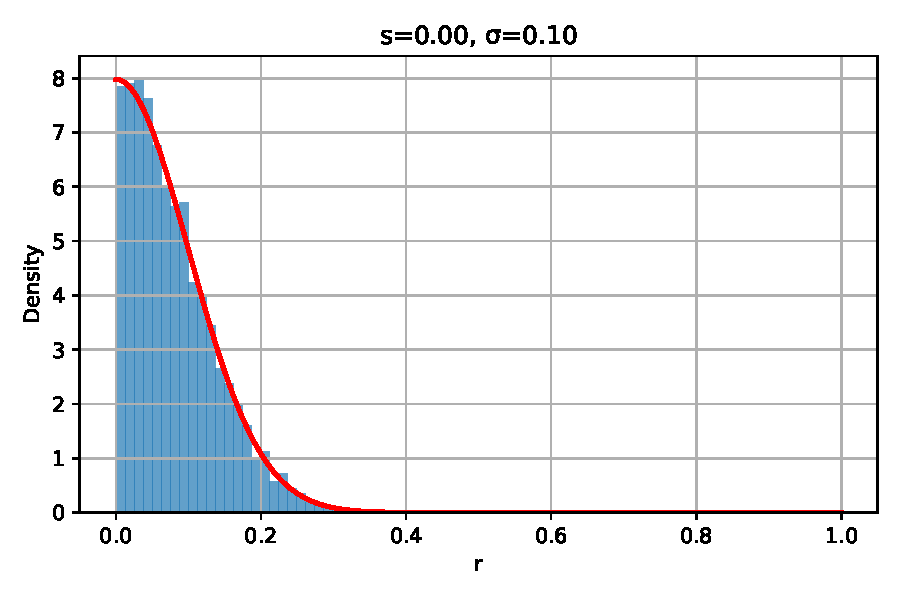
\includegraphics[width=0.32\linewidth]{pics/sampler/s00_step0.pdf} &
    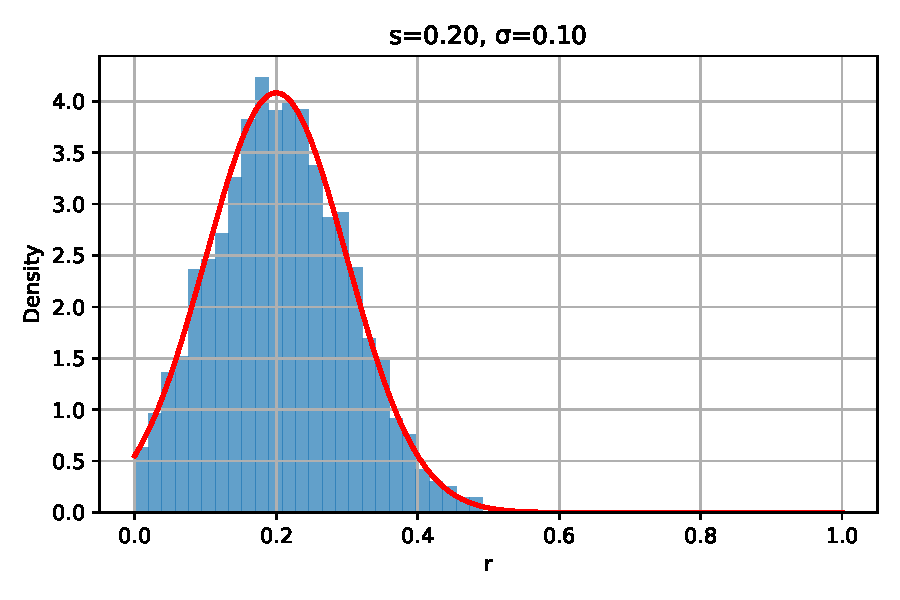
\includegraphics[width=0.32\linewidth]{pics/sampler/s20_step0.pdf} &
    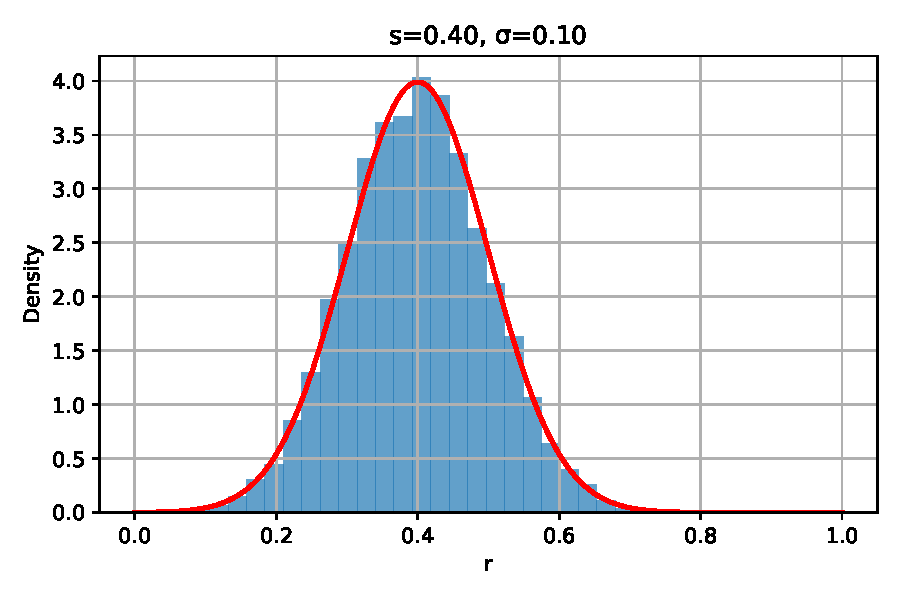
\includegraphics[width=0.32\linewidth]{pics/sampler/s40_step0.pdf} \\
    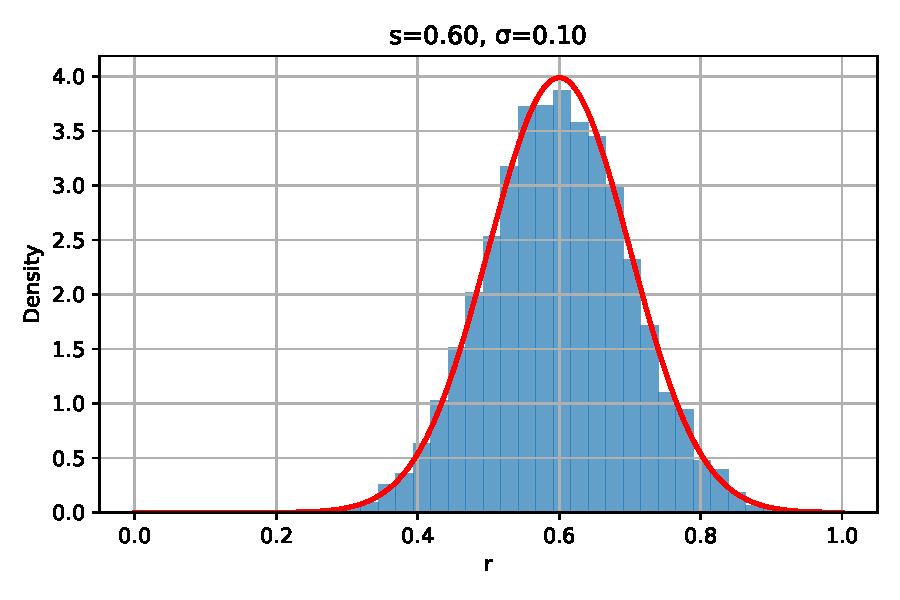
\includegraphics[width=0.32\linewidth]{pics/sampler/s60_step0.pdf} &
    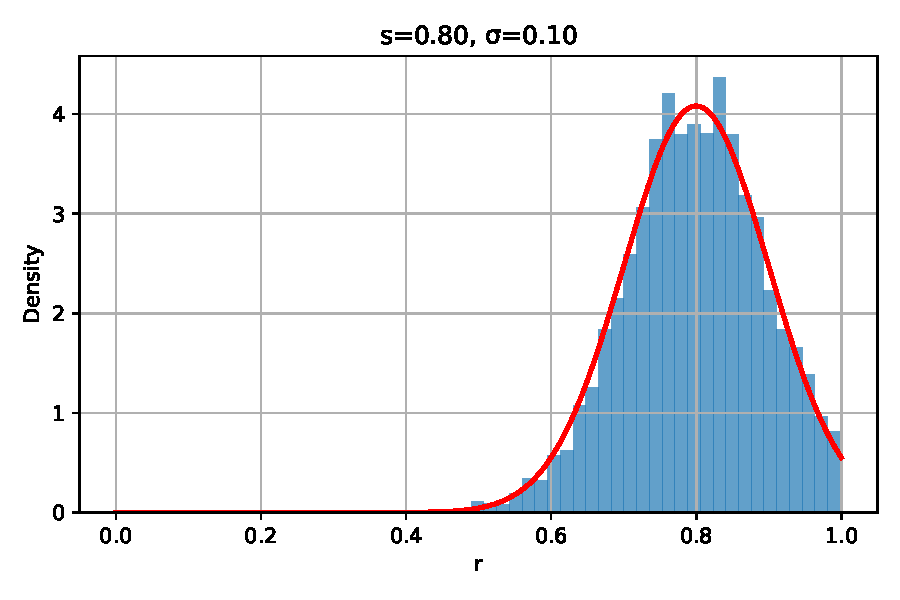
\includegraphics[width=0.32\linewidth]{pics/sampler/s80_step0.pdf} &
    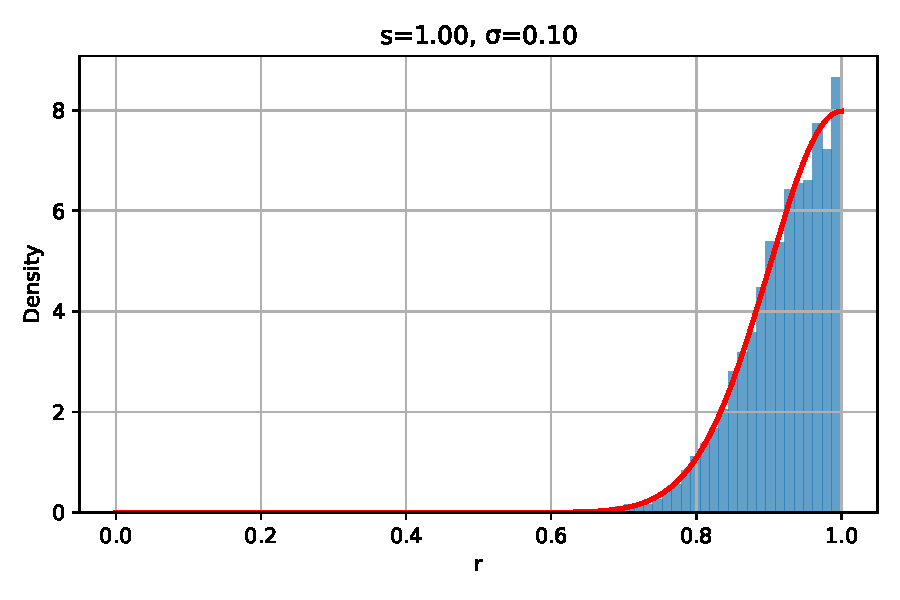
\includegraphics[width=0.32\linewidth]{pics/sampler/s100_step0.pdf} \\
  \end{tabular}
  \caption{Sampling prior \(p(r\mid s)\) on \([0,1]\) for various center values \(s\) with scale \(\sigma=0.1\).}
  \label{fig:trunc_gauss_sigma_0.1}
\end{figure}

%—— figure for σ=0.05 ——%
\begin{figure}[!htbp]
  \centering
  \begin{tabular}{ccc}
    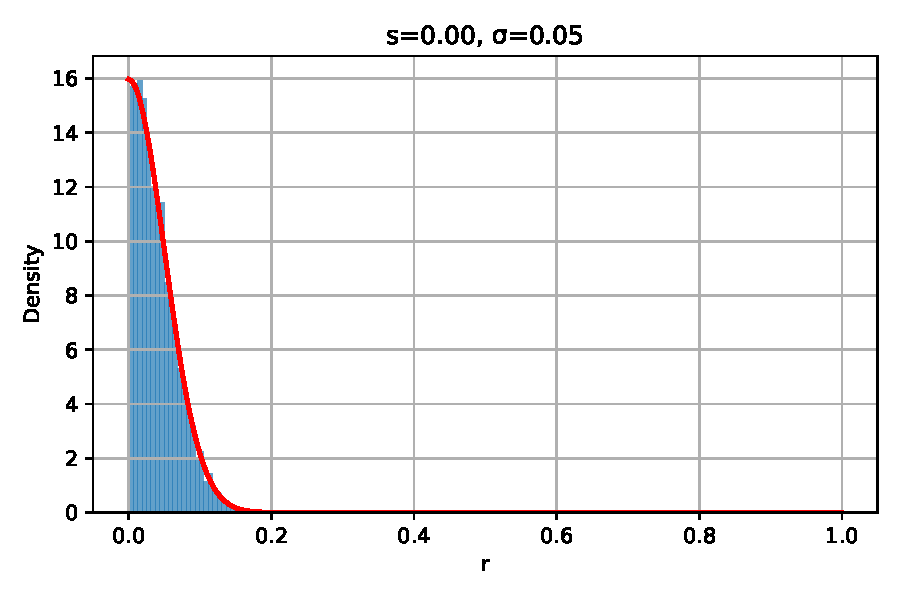
\includegraphics[width=0.32\linewidth]{pics/sampler/s00_step69.pdf} &
    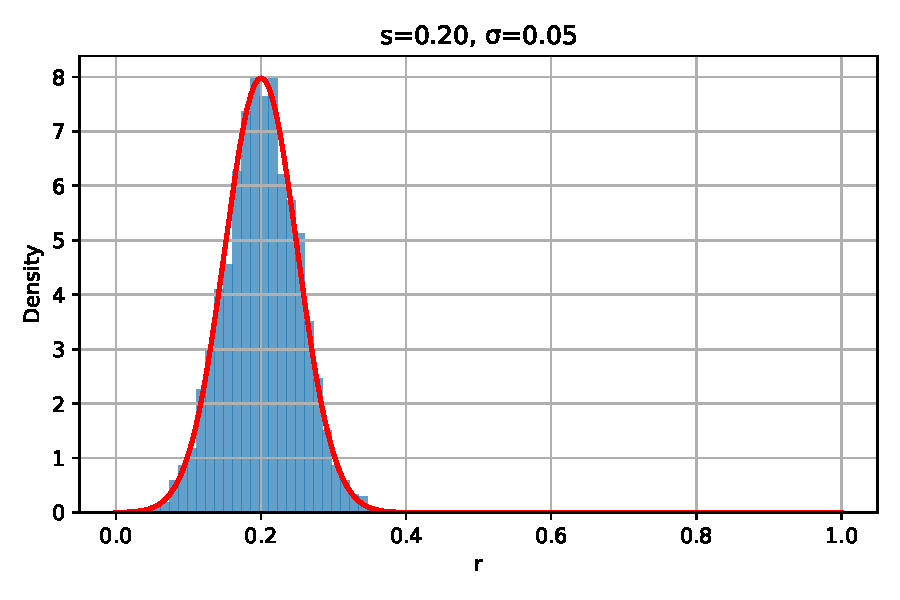
\includegraphics[width=0.32\linewidth]{pics/sampler/s20_step69.pdf} &
    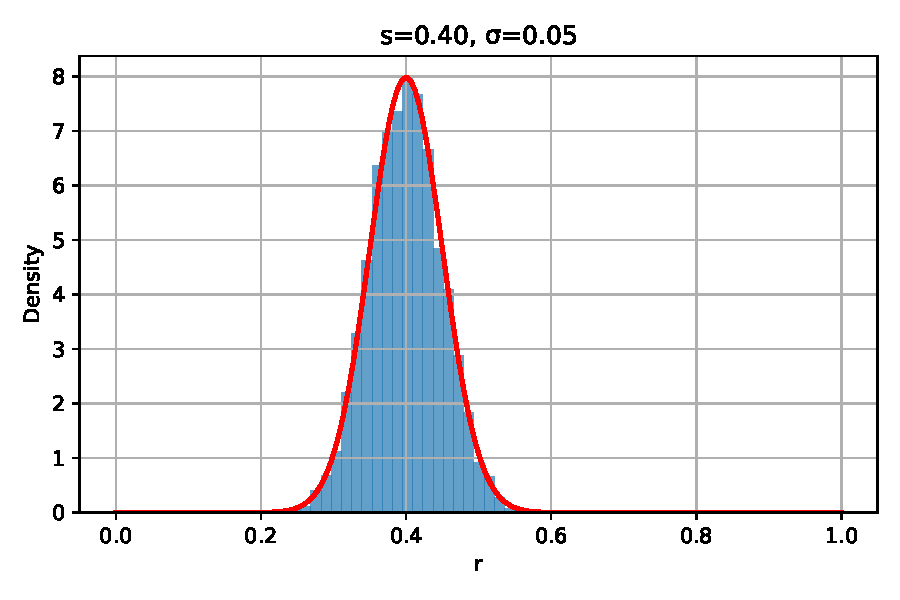
\includegraphics[width=0.32\linewidth]{pics/sampler/s40_step69.pdf} \\
    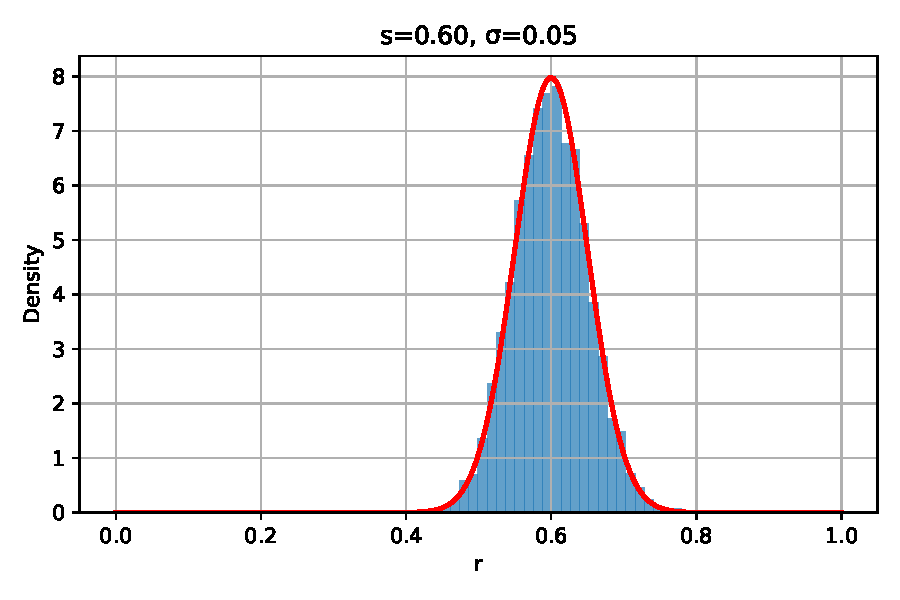
\includegraphics[width=0.32\linewidth]{pics/sampler/s60_step69.pdf} &
    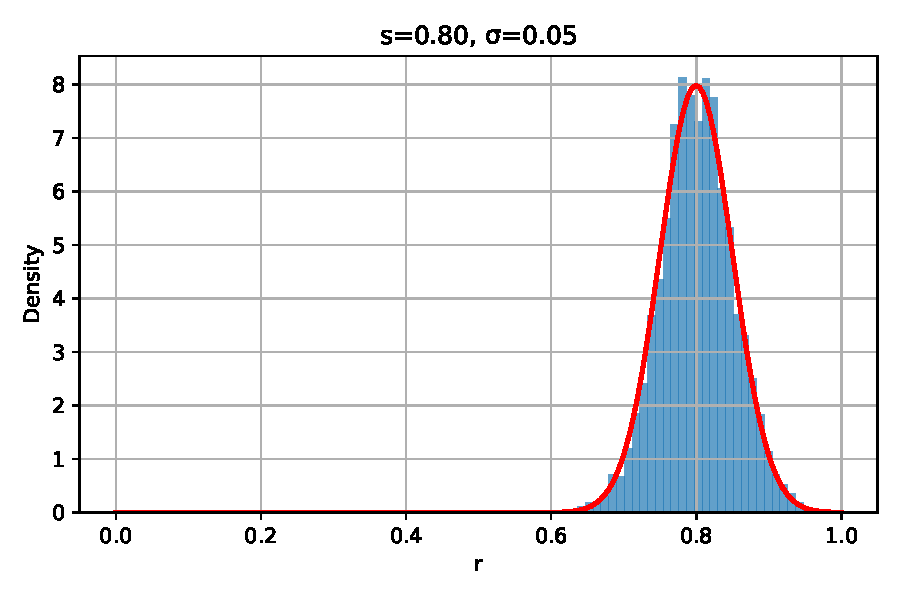
\includegraphics[width=0.32\linewidth]{pics/sampler/s80_step69.pdf} &
    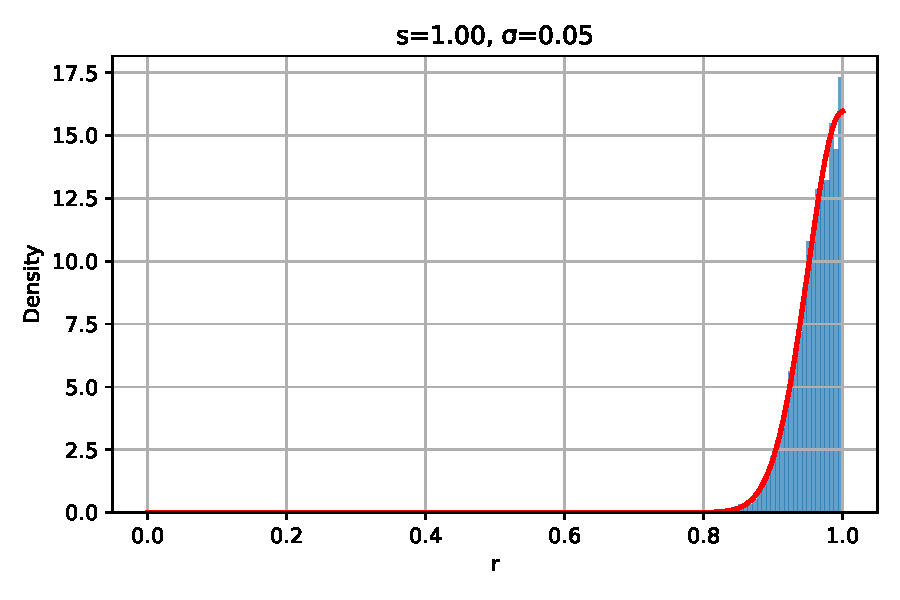
\includegraphics[width=0.32\linewidth]{pics/sampler/s100_step69.pdf} \\
  \end{tabular}
  \caption{Sampling prior \(p(r\mid s)\) on \([0,1]\) for various center values \(s\) with scale \(\sigma=0.05\).}
  \label{fig:trunc_gauss_sigma_0.05}
\end{figure}

%—— figure for σ=0.01 ——%
\begin{figure}[!htbp]
  \centering
  \begin{tabular}{ccc}
    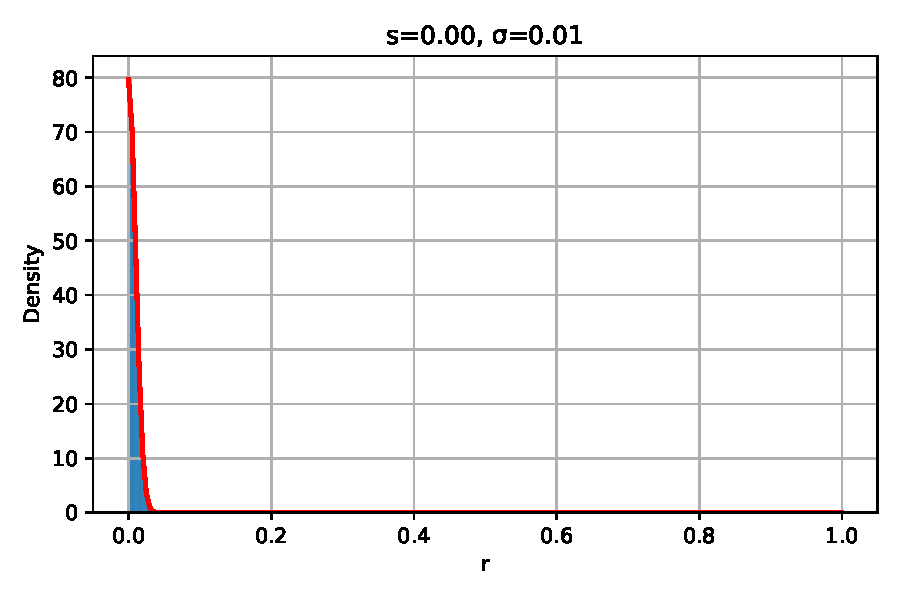
\includegraphics[width=0.32\linewidth]{pics/sampler/s00_step229.pdf} &
    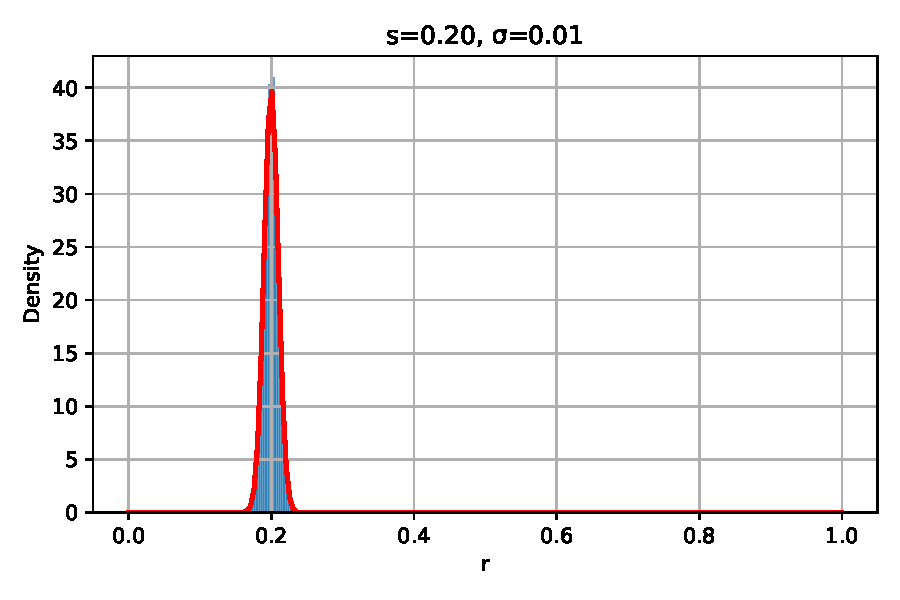
\includegraphics[width=0.32\linewidth]{pics/sampler/s20_step229.pdf} &
    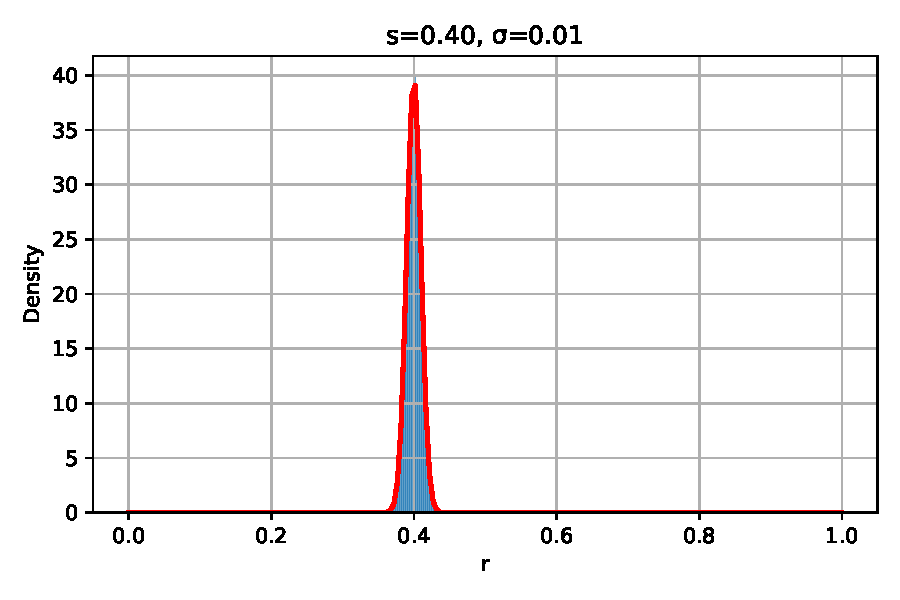
\includegraphics[width=0.32\linewidth]{pics/sampler/s40_step229.pdf} \\
    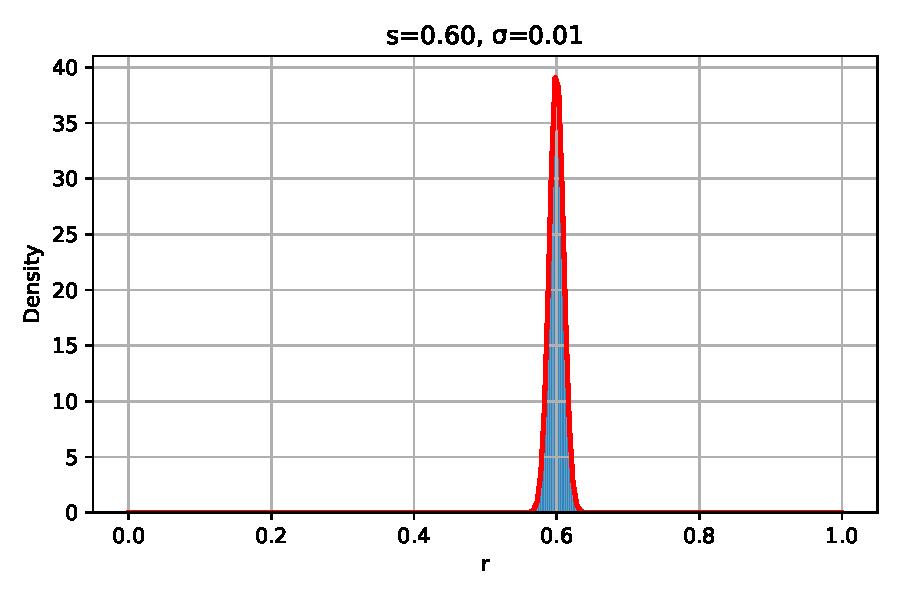
\includegraphics[width=0.32\linewidth]{pics/sampler/s60_step229.pdf} &
    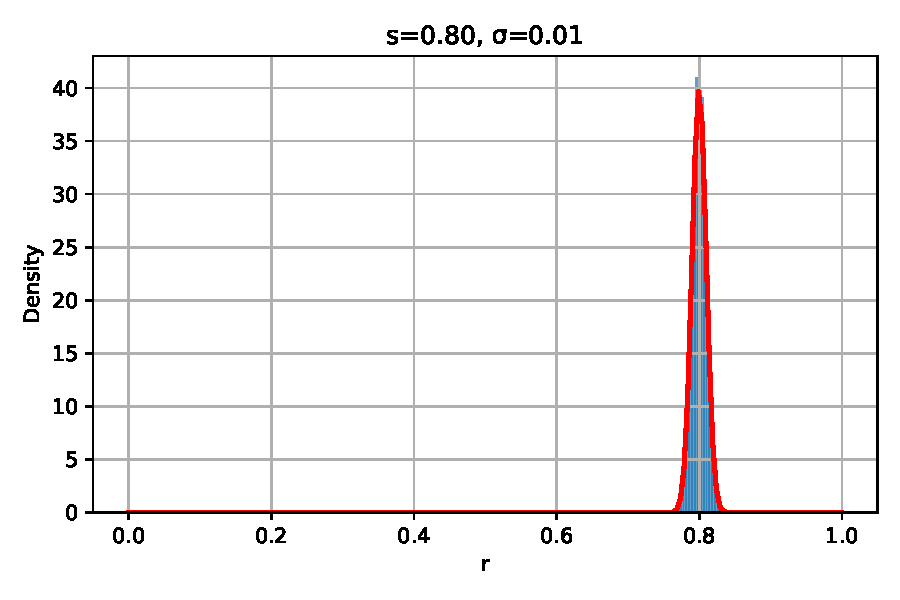
\includegraphics[width=0.32\linewidth]{pics/sampler/s80_step229.pdf} &
    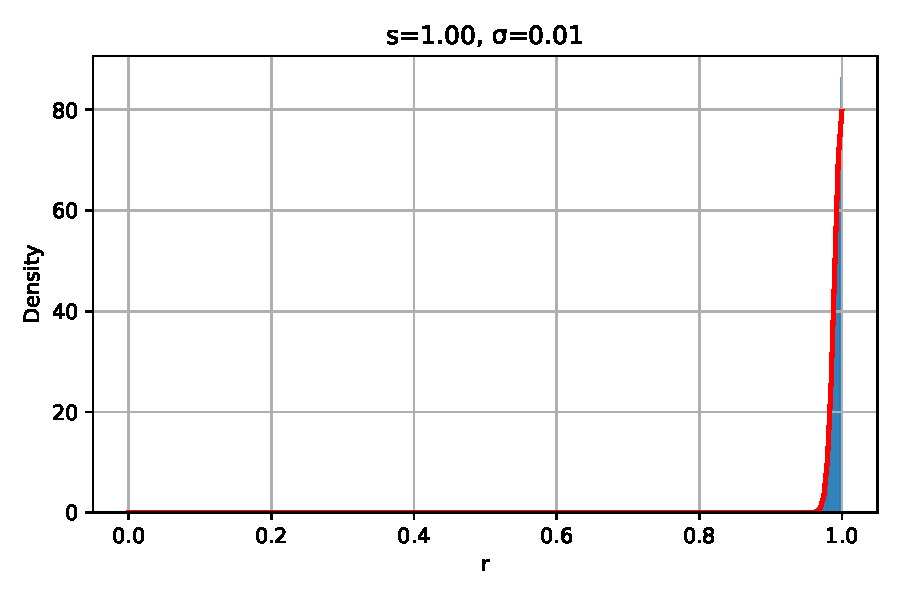
\includegraphics[width=0.32\linewidth]{pics/sampler/s100_step229.pdf} \\
  \end{tabular}
  \caption{Sampling prior \(p(r\mid s)\) on \([0,1]\) for various center values \(s\) with scale \(\sigma=0.01\).}
  \label{fig:trunc_gauss_sigma_0.01}
\end{figure}

\section{Additional experimental results}
\label{appendix:additional-results}
\paragraph{Additional result on MNIST}
The purpose of this experiment is to investigate the effect of compute budget on data selection within the MNIST dataset. We vary the compute budget in terms of total forward counts (10 000, 20 000, 50 000 and 100 000). At each budget we compare four sampling strategies—random, PBCS, CADS-E and our Bilevel-CADS.
As shown in Table~\ref{tab:mnist_vary_budget}, our Bilevel-CADS consistently outperforms all baselines in all compute budgets.
\begin{table}[!htbp]
  \centering
  \caption{Results on MNIST with various compute budgets.}
  \label{tab:mnist_vary_budget}
  \resizebox{0.6\linewidth}{!}{%
    \begin{tabular}{@{}lccccc@{}}
      \toprule
      \multirow{2}{*}{Method} & \multicolumn{4}{c}{Compute budget} & \multirow{2}{*}{Average} \\
      \cmidrule(lr){2-5}
                              & 10,000 & 20,000 & 50,000 & 100,000 & \\
      \midrule
        Random                  & 87.36          & 88.05          & 87.71          & 87.24          & 87.59                    \\
      PBCS                    & 89.61          & 90.48          &  90.96    & 90.41    & 90.37                    \\
      CADS-E                  & {\ul 90.62}    & {\ul 91.48}    & {\ul 92.45}          & {\ul 93.17}          & {\ul 91.93}              \\
      Bilevel-CADS            & \textbf{90.70} & \textbf{92.44} & \textbf{93.09} & \textbf{93.61} & \textbf{92.46}           \\ \bottomrule
    \end{tabular}%
  }
\end{table} 
\section{Time efficiency analysis}
\label{appendix:time_efficiency}

\subsection{Computational complexity compare to standard bilevel optimization}  
We compare the per‐iteration cost of our single‐epoch inner loop against the full‐training inner loop used in bilevel-CADS, and then account for the one-time cost of fitting the loss estimator $l(|\bm m|)$.

Let
\begin{itemize}
  \item $|\mathcal D|$ be the size of the training set,  
  \item $T_{\mathrm{ep}}=O(|\mathcal D|)$ the cost of one full epoch (one forward+backward pass),  
  \item $N$ the number of epochs used by bilevel-CADS in its inner optimizer,  
  \item $K$ the number of subsets sampled per outer iteration,  
  \item $|\bm m|$ the average subset size,  
  \item $M$ the total number of outer iterations in a run.
\end{itemize}

\paragraph{Bilevel-CADS inner solve (per outer step)}  
\[
\mathrm{Cost}_{\rm bilevel}
\;=\;
K \times N \times T_{\mathrm{ep}}
\;=\;
O\bigl(KN\,|\mathcal D|\bigr).
\]

\paragraph{Our CADS-E/S inner loop (per outer step, ignoring estimator)}  
\[
\mathrm{Cost}_{\rm CADS}^{\rm base}
\;=\;
K \times T_{\mathrm{ep}}
\;=\;
O\bigl(K|\mathcal D|\bigr).
\]

\paragraph{Estimator fitting overhead}  
To fit the mapping $l(|\bm m|)$ we train 8 models for $N$ epochs each (As detailed in ~\ref{appendix:gaussian}), incurring a one‐time cost  
\[
\mathrm{Cost}_{\rm est}
\;=\;
8 \times N \times T_{\mathrm{ep}}.
\]
Amortized over $M$ outer steps, this adds  
\[
\frac{\mathrm{Cost}_{\rm est}}{M}
\;=\;
\frac{8\,N\,T_{\mathrm{ep}}}{M}
\]
to each iteration.

\paragraph{Total CADS cost (amortized)}  
\[
\mathrm{Cost}_{\rm CADS}
\;=\;
K\times T_{\mathrm{ep}}
\;+\;
\frac{8\,N\,T_{\mathrm{ep}}}{M}
\;=\;
T_{\mathrm{ep}}\Bigl(K + \tfrac{8\,N}{M}\Bigr).
\]

\paragraph{Speed-up factor}  
\[
\frac{\mathrm{Cost}_{\rm bilevel}}{\mathrm{Cost}_{\rm CADS}}
\;=\;
\frac{K\,N\,T_{\mathrm{ep}}}{T_{\mathrm{ep}}\bigl(K + \tfrac{8\,N}{M}\bigr)}
\;=\;
\frac{K\,N}{K + 8\,N/M}.
\]
In our experiments \(K = 5\) and \(M = 100\), giving
\[
\frac{\mathrm{Cost}_{\rm bilevel}}{\mathrm{Cost}_{\rm CADS}}
\;=\;
\frac{1}{1/N + 0.016}.
\]
In practice, larger $N$ yields an even greater speed-up.

\subsection{Empirical Validation}  

We measure end-to-end wall-clock time of bilevel-CADS and CADS-E on MNIST as a function of compute budget $C$ (total epochs).  We sweep $C$ over $\{5,50,100,200,500,1000,2000,5000\}$ and record the runtime of each method under identical hardware. Figure~\ref{fig:time_efficiency_empirical} confirms a roughly linear scaling for both methods, with CADS-E exhibiting a much smaller slope.


\subsection{Analysis of Selection Algorithm Runtime}
\label{appendix:runtime_analysis}

A potential concern regarding our method is that the runtime of the selection algorithm may scale with the number of sampled subsets (\(K\)), which could offset the computational efficiency gains. We address this concern by highlighting several key aspects of our approach.

\paragraph{Minimal Sampling for Practical Implementation}
Our policy gradient approach for coreset selection requires only a small number of samples (\(K\)) to ensure training stability. For instance, the comparable PBCS method \cite{ds_bi_zhou2022probabilistic} utilizes \(K=1\) for all its experiments. Our results show that using \(K=2\) is sufficient to achieve strong performance while maintaining high computational efficiency. In cases where smaller \(K\) values might lead to higher gradient variance (e.g., in more complex problems), this can be mitigated using established variance reduction techniques. A common approach is to use a self-critical baseline, which adjusts the reward signal as follows:
\begin{equation}
\label{eq:variance_reduction}
\tilde{\mathcal{L}}(S_i) = \mathcal{L}(S_i) - \frac{1}{K} \sum_{j=1}^{K} \mathcal{L}(S_j).
\end{equation}

\paragraph{Amortized Cost of Coreset Selection}
It is important to emphasize that the core contribution of this work is the introduction of computational budget constraints into the coreset selection process, rather than optimizing the selection runtime itself. Once generated, a coreset is a reusable asset that can be applied across various training scenarios, different model architectures, and subsequent experiments. Consequently, the initial computational investment in the selection process is amortized over these multiple uses. This makes the selection efficiency a secondary consideration compared to the quality and utility of the resulting budget-constrained coreset.


\begin{figure}[!htbp]  
  \centering  
  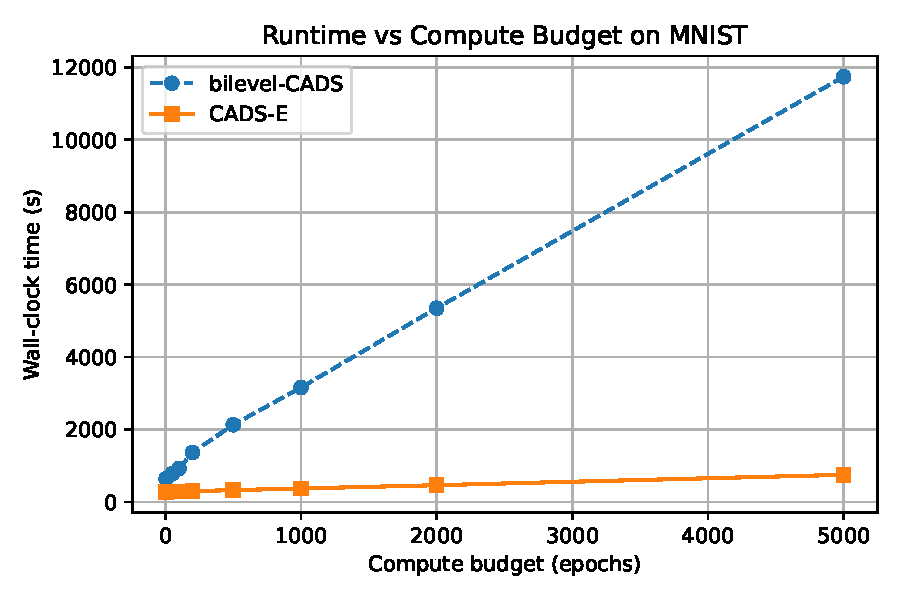
\includegraphics[width=0.6\textwidth]{pics/runtime_vs_budget.pdf}  
  \caption{Wall-clock runtime vs.\ compute budget $C$ for bilevel-CADS (dashed) and CADS-E (solid), MNIST.}  
  \label{fig:time_efficiency_empirical}  
\end{figure}  


\section{Scalability to Other Bilevel Optimization Problems}
\label{appendix:scala2other}
CADS is designed to address a fundamental challenge in bilevel optimization: scenarios where the inner-level problem's convergence is hindered by computational budget constraints. Many practical bilevel problems suffer from this issue, where traditional methods that assume unlimited computational resources for inner-level convergence often fall short. We have also successfully applied a CADS-like method to resource-intensive diffusion models, demonstrating its potential beyond the scope of this work. The scalability of CADS to other bilevel problems primarily depends on the following factors:

\paragraph{Applicability Conditions}
The core premise of CADS is most relevant when the inner-level optimization is computationally expensive and cannot be fully converged. Our approach provides a framework to handle such resource-constrained scenarios, which are common in real-world applications but often overlooked by conventional methods.

\paragraph{Loss Estimation Accuracy}
The effectiveness of CADS in a new domain hinges on the accuracy of the loss estimator. As demonstrated in our analysis of loss estimation generalization, the proposed estimator maintains relatively stable predictive performance across the diverse experimental domains explored in this paper. This stability suggests that similar performance may be achievable in other domains with comparable data characteristics.

\paragraph{Validation Framework for New Domains}
To adapt CADS to a new bilevel optimization problem, we propose the following validation framework:
\begin{itemize}
\item \textbf{Loss Estimator Generalization Assessment.} Before full-scale implementation, it is crucial to assess whether the data distribution characteristics of the new domain can be reliably predicted. This can be achieved by conducting experiments similar to our generalization evaluation to validate the feasibility of loss estimation.
\item \textbf{Domain-Adaptive Estimator Design.} While our current estimator is effective for data selection problems, different bilevel scenarios might benefit from specialized estimators. The architecture of the loss estimator should be tailored to the specific requirements and data characteristics of the target domain to ensure optimal performance.
\end{itemize}
\section{Limitations and Future Work}
\label{appendix:limitation}
Similar to existing methods, our approach is based on standard training methodologies, but in the industry, large language models incorporate numerous engineering optimizations. Consequently, our budget is likely proportional to theirs, rather than perfectly aligned. For instance, in sparse mixture of experts (MoE), the budget is determined by model capacity and routing complexity, whereas we measure performance by the number of forward passes. This measurement may not fully correspond with the budget metrics used in industry. However, we firmly believe that our methods are applicable in industrial contexts; we simply need to adjust the budget measurements accordingly.

\section{Licenses for existing assets}
\label{appendix:license}
We rely on several public datasets and open-source libraries, and all original authors are properly credited and their licenses fully respected. The vision benchmarks we employ are MNIST (public domain), CIFAR-10 (MIT License) and DomainNet (CC BY-NC-SA 4.0). Our instruction-tuning corpora are summarized in Table \ref{tab:stat_data}, with licenses ranging from Apache 2.0 to various Creative Commons and MIT terms. On the software side, we build atop PyTorch and torchvision (BSD 3-Clause), SciPy (BSD), and HuggingFace Transformers (GPT-2, Apache 2.0); ResNet models are taken from torchvision (BSD 3-Clause). We confirm that every dataset and code dependency is used in accordance with its license and citation requirements.